\section{Single planet retrieval}
\label{sec:singles}

For the evaluation of the ability of the RNN-based algorithms to retrieve single planets with multiple transit signals, we apply the RNN from previous sections to light curves in the LCSim-Single data set. Subsequently, we use PTS-Fold and PTS-Peak to determine the period and epoch of a maximum of three candidate signals per light curve. Both algorithms provide for each candidate a corresponding detection score, as described in Section \ref{sec:algorithm}, which is used to set a detection threshold. A detection is counted as correct if the estimated period is correct with a 1\% error margin, and the estimated epoch is within the duration of the first transit in the light curve.

As baseline we use the standard BLS algorithm, as implemented in the \texttt{astropy} package\footnote{\url{https://docs.astropy.org/en/stable/timeseries/bls.html}. Accessed: 18-08-2021.}. We set a detection threshold on the SDE of each candidate in the BLS periodogram, and recursively apply the method to search for a maximum of three potential signals per light curve, each time masking the previous signal that was found. The algorithm is applied to detrended light curves using sliding median filters of varying lengths, i.e. 6, 12, and 24 hours.

Figure \ref{fig:single_pr} shows that a 12-hour window works best for detrending in combination with BLS for this task, which is in line with the results from \cite{hippke2019wotan}. Moreover, the results show that the BLS algorithm outperformed the RNN-based detection algorithms in this experiment. Among the RNN-based algorithms tested, PTS-Fold performed best, which was as expected because it does not rely on distinct peaks in the PTS as opposed to PTS-Peak. The performances of the best algorithms are further inspected in Figure \ref{fig:single_transit}. This figure shows, in line with our monotransit experiment, that towards larger periods, i.e. fewer transit signals, the performance of BLS drops faster than that of the RNN-based algorithm. This suggests that if there is periodicity in the signal, BLS remains dominant over the RNN. However, if the periodicity is lacking, the RNN is the preferred method. Table \ref{tab:single_AnotB} presents the number of planets retrieved by the methods, including the number of planets that were detected by one algorithm and not by the other.

The RNN-based algorithm required a longer computation time in this case than in the monotransit case. To obtain the PTS of each of the 5000 light curves still required only a few minutes on a GPU, but the determination of the periodicity of potential signals added more to the necessary computation time. PTS-Peak required only 5 minutes on a CPU. PTS-Fold on the other hand, took about 1.5 hours. Still, PTS-Fold was faster than BLS which took over 3 hours of computation time. The computation times are in line with the relative performances of each method in this task. Nevertheless, it is noteworthy that PTS-Peak retrieved 20 planets that BLS was not able to find at a precision of 0.5, while using less than 35 times its computation time.


\begin{figure}
    \centering
    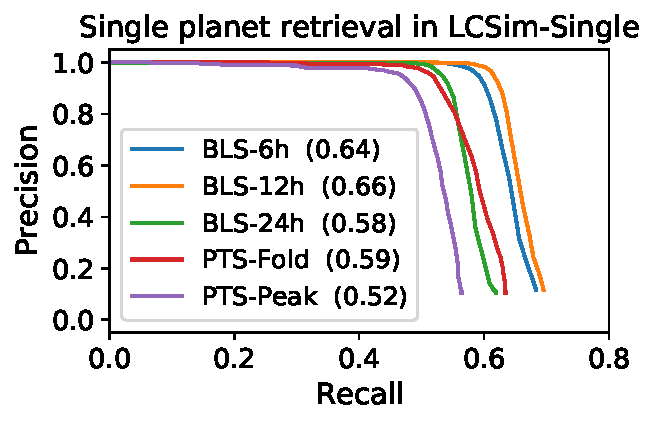
\includegraphics[width=0.35\linewidth]{Experiments/Figures/Singles/single_pr.pdf}
    \caption{Precision-recall curves for different methods in the task of detecting repeating transit signals of a single planet. The average precision is given between brackets.}
    \label{fig:single_pr}
\end{figure}


\begin{figure}
    \centering
    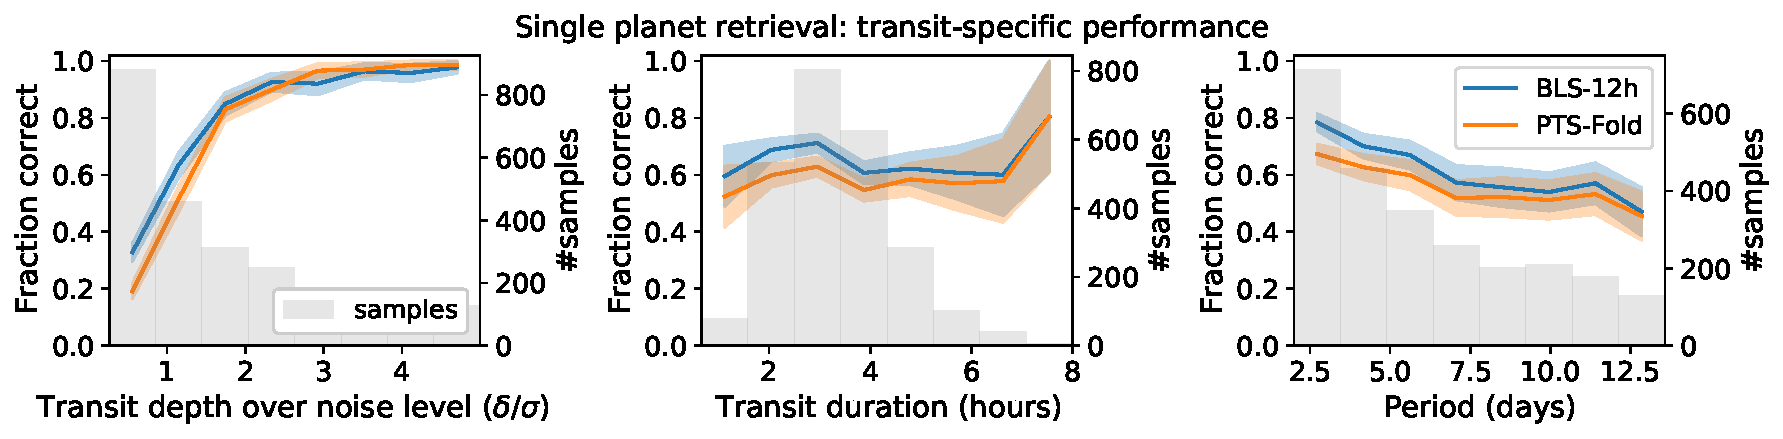
\includegraphics[width=\linewidth]{Experiments/Figures/Singles/single_transit_specific.pdf}
    \caption{The ability of the presented methods to retrieve planets within the given parameter ranges. A detection threshold was set closest to a corresponding detection precision of 0.5. PTS-Peak is not shown because it behaves similarly but worse than PTS-Fold and would therefore only clutter the image. Filled regions show the Wilson score interval \citep{wilson1927probable}, which approximates the 95\% confidence interval of the performance per bin.}
    \label{fig:single_transit}
\end{figure}



\begin{table}[h]
\label{tab:single_AnotB}
\centering
\begin{tabular}{@{}lrlrlrl@{}}
\toprule
             & \multicolumn{2}{c}{PTS-Fold} & \multicolumn{2}{c}{PTS-Peak} & \multicolumn{2}{c}{BLS-12h} \\ \midrule
             & 1480      & (1.00, 0.59)     & 1333      & (1.00, 0.53)     & 1655     & (1.00, 0.66)     \\
not PTS-Fold & -         &                  & 7         & (0.01, 0.00)     & 224      & (0.14, 0.09)     \\
not PTS-Peak & 154       & (0.10, 0.06)     & -         &                  & 342      & (0.21, 0.14)     \\
not BLS-12h  & 49        & (0.03, 0.02)     & 20        & (0.02, 0.01)     & -        &                  \\ \bottomrule
\end{tabular}
\caption{The absolute and relative number of correct detections in the task of retrieving planets with multiple transit signals, where the detection thresholds are set closest to a corresponding detection precision of 0.5. The data contained a total of 2500 planets.}
\end{table}